\documentclass{beamer}
%
% Choose how your presentation looks.
%
% For more themes, color themes and font themes, see:
% http://deic.uab.es/~iblanes/beamer_gallery/index_by_theme.html
%
\mode<presentation>
{
  \usetheme{JuanLesPins}      % or try Darmstadt, Madrid, Warsaw, ...
  \usecolortheme{default} % or try albatross, beaver, crane, ...
  \usefonttheme{default}  % or try serif, structurebold, ...
  \setbeamertemplate{navigation symbols}{}
  \setbeamertemplate{caption}[numbered]
} 

\usepackage[ngerman]{babel}
\usepackage[utf8x]{inputenc}
\usepackage{amsmath}
\usepackage{graphicx}
\usepackage{csquotes}
\usepackage{nicematrix}
\usepackage{bbm}
\usepackage{mathtools} 

% norm
\usepackage{physics}

\title{Benign Overfitting}
\date{16. December 2021}
\author{Linus Boehm, Jurek Rostalsky}


\begin{document}
\maketitle

\begin{frame}{Content}
\tableofcontents
\end{frame}

\section{Setting}

\begin{frame}{Intruduction}
\begin{itemize}
	\item Overfitting: fit every training example perfectly
	\item assume that the dimension of parameter space is large enough that a perfect hit is guaranteed 
	\item require more parameters than the sample size in order to fit exactly
	\item the solution might be underdetermined, so there might be many interpolating solutions
	\item target: find a characterization when overfitting is benign
\end{itemize}
\end{frame}

\section{Benign Overfitting - Theory}

\begin{frame}{Linear Regression}
	
The linear regression problem depends on the optimal parameters $\theta^*$ and the covariance $\Sigma$ of the covariates x.

\begin{center}
\begin{block}{Linear-Regression}
The problem of finding a parameter vector \(\theta^\ast \in \mathbb{H}\) with 
$\theta^\ast = arg \min\limits_\theta \mathbb{E}\left((y - x^T \theta)^2\right)$
is called \textbf{linear regression}
\end{block}
\begin{block}{covariance-matrix}
$\Sigma = \mathbb{E}\left(\left(x - \mathbb{E}(x)\right)\left(x - \mathbb{E}(x)\right)^T\right) =  \mathbb{E}(xx^T)$
\end{block}
\end{center}
\end{frame}

\begin{frame}{Definitions}
\begin{center}
\begin{block}{Excess risk}
	$\mathbb{E}_{x,y}$ denotes the conditional expectation , then define:
	$R(\theta):= \mathbb{E}_{x,y}[(y - x^T\theta)^2 - (y - x^T\theta^*)^2]$
\end{block}
\begin{block}{Effective Ranks}
	For the covariance operator $\Sigma$, define $\lambda_i = \mu_i(\Sigma)$ for $i = 1,2,...$ . Whereby: $\mu_1(\Sigma) \geq \mu_2(\Sigma) \geq ...$ . If $\sum\limits_{i=1}^\infty \lambda_i < \infty$ and $\lambda_{k+1} > 0$
	define: 
	$r_k(\Sigma) = \frac{\sum_{i>k}\lambda_i}{\lambda_{k+1}} ,\hspace*{1cm}
	R_k(\Sigma) = \frac{(\sum_{i>k}\lambda_i)^2}{\sum_{i>k}\lambda_i^2}$
\end{block}
\end{center}
\end{frame}

\begin{frame}{Definitions}
	\begin{center}
		\begin{block}{Minimum Norm estimator}
			For given samples \(X \in \mathbb{H}^n, y \in \mathbb{R}^n\). The \textbf{minimum norm estimator} \(\theta\) is the solution of:
			\hspace*{0.4 cm}$\hat{\theta} = arg \min\limits_{\theta} \norm{\theta}^2$\newline such that  $\norm{X \theta - y}^2 = \min\limits_\beta \norm{X \beta - y}^2$\\
			\hspace*{3 cm} $\hat{\theta} = X^T(XX^T)^{-1}y$
		\end{block}
	\end{center}
\end{frame}


\begin{frame}{Theorem(1)}
	
For any $\sigma_x$ there are $b,c,c_1 > 1$, for which the following holds.
Define:
\begin{align*}
k^* = \min \{k \geq 0: r_k(\Sigma) \geq bn\},
\end{align*}
	
Where the minimum of the empty set is defined as $\infty$. Suppose $\delta < 1$ with $\log(\frac{1}{\delta}) < n/c$. If $k^* \leq n/c_1$, then $\mathbb{E}R(\hat{\theta}) \leq \delta^2/c.$ Otherwise,\\
	
	
$R(\hat{\theta}) \leq c(\norm{\theta^*}^2\norm{\Sigma}\max{\sqrt{\frac{r_0(\Sigma)}{n}},\frac{r_0(\Sigma)}{n},\sqrt{\frac{\log(1/\delta)}{n}}}) 
$\newline \hspace*{0.85 cm}$+ c\log(\frac{1}{\delta})\sigma_y^2\left(\frac{k^*}{n} + \frac{n}{R_{k^*(\Sigma)}}\right)$\\

with probability at least $1 - \delta$

\end{frame}


\begin{frame}{Theorem(1)}

\begin{align*}
	\mathbb{E}R(\hat{\theta}) \geq \frac{\sigma^2}{c} \left(\frac{k^*}{n} + \frac{n}{R_{k^*(\Sigma)}}\right)
\end{align*}


Moreover there are universal constants $a_1.a_2,n_0$ such that $\forall n \geq n_0, \forall \Sigma, \forall t \geq 0$ there is a $\theta^*$ with $\norm{\theta^*} = t$ such that for $x \sim N(0,\Sigma)$ and $y|x \sim N(x^T\theta^*,\norm{\theta^*}^2\norm{\Sigma})$, with probability at least $1/4$,
	

\begin{align*}
	R(\hat{\theta})\geq \frac{1}{a_1}\norm{\theta^*}^2\norm{\Sigma}\mathbbm{1}_{\left[\frac{r_0(\Sigma)}{n\log(1+r_0(\Sigma))} \geq a_2\right]}
\end{align*}

\end{frame}

\begin{frame}{Conclusions Theorem(1)}
\begin{itemize}
\item $r_0(\Sigma)$ should be small compared to the sample size n
\item $R_{k^*}(\Sigma)$ should be large compared to n
\item $\frac{k^*}{n}$ should be small
\end{itemize}
\vspace*{0.5 cm}

$\rightarrow $ the number of non-zero eigenvalues should be large compared \hspace*{0.4 cm} to n, but they should have a small sum

\end{frame}


\begin{frame}{Proof}

\begin{center}
\begin{block}{Theorem}
	\begin{align*}
	R(\hat{\theta)} & \leq 2(\theta^*)^TB\theta^* + 2\epsilon^TC\epsilon\\\\
	B & = (I - X^T(XX^T)^{-1}X)\Sigma(I - X^T(XX^T)^{-1}X),  \\
	C & = (XX^T)^{-1}X\Sigma X^T(XX^T)^{-1}
	\end{align*}
\end{block}
\end{center}
\end{frame}

\begin{frame}{Proof}
\end{frame}

\begin{frame}{Proof}
\end{frame}

\begin{frame}{Proof}
\end{frame}

\begin{frame}{Proof}
\end{frame}

\begin{frame}{Proof}
\end{frame}

\begin{frame}{Proof}
\end{frame}


\begin{frame}{Theorem(2)}
1. If $\mu_k(\Sigma) = k^{-\alpha}ln^{-\beta}(k+1), $ then $\Sigma$ is benign iff $\alpha = 1$ and $\beta > 1$\\

\vspace*{0.3 cm} 2. If
\begin{equation*}
	\mu(\Sigma_n) = \begin{cases}
		\gamma_k + \epsilon_n & if \, k \leq p_n \\
		0 & otherwise
	\end{cases}
\end{equation*}

and $\lambda_k = \Theta(exp(-k/\tau))$, then $\Sigma_n$ is benign iff $p_n = \omega(n)$ and $ne^{o(n)} = \epsilon_np_n = o(n).$
\end{frame}


\begin{frame}{Conclusions Theorem(2)}
	benign overfitting if:
\begin{itemize}
	\item Part 1: eigenvalues of $\Sigma$ decay slowly enough that sum to remain finit
	\item Part 2: dimension is large compared to sample size and isotropic component is almost as small as  exponential
\end{itemize}
\end{frame}

\begin{frame}{Proof-Ideas for Theorem(2) Part 1}
\begin{itemize}
	\item idea: use Theorem 4
	\item $\Sigma$ benign if $\lim\limits_{n \rightarrow \infty}\frac{r_0(\Sigma_n)}{n} = \lim\limits_{n \rightarrow \infty}\frac{k^*_n}{n} = \lim\limits_{n \rightarrow \infty}\frac{n}{R_{k^*_n}(\Sigma_n)} = 0$
\end{itemize}
\begin{center}
	\begin{block}{Help-Theorem 1}
	Consider some positive summable sequence ${\lambda_i}_{i=1}^\infty $ and for i integer, denote \hspace*{2.3cm} $r_i := \lambda_{i+1}^{-1}\sum\limits_{j>i}\lambda_j$\\
	Then $r_i >1$. Moreover for any positive sequence ${u_i}$ such that $\sum\limits_{i=0}^\infty u_i^{-1} = \infty$ and for every $i \hspace*{0.1cm} u_i>1$ there exist positive sequence ${\lambda_i}$ such that $r_i \equiv \lambda_i$ (unique up to constant multiplier). The sequence is:\\
	\hspace*{3.4 cm}$\lambda_k = u_{k-1}^{-1}\prod\limits_{i=0}^{k-2}(1-u_i^{-1})$
	\end{block}
\end{center}
\end{frame}


\begin{frame}{Proof-Ideas for Theorem(2) Part 1}
	\begin{center}
		\begin{block}{Help-Theorem 2}
			Suppose b is some constant and $k^*(n) = \min\{k: r_k \geq bn\}$. Suppose also that the sequence ${r_n}$ is increasing. Then , as n goes to infinity, $k^*(n)/n$ goes to zero if and only if $r_n/n$ goes to infinity
		\end{block}
	\end{center}

\begin{center}
	\begin{block}{Help-Theorem 3}
		Suppose the sequence ${r_i}$ is increasing and $r_n/n \rightarrow \infty$ as $n \rightarrow \infty$. Then a sufficient condition holds for $\frac{n}{R_{k^*(n)}} \rightarrow 0$ is \\
		\hspace*{3cm}$r_k^{-2} = o(r_k^{-1} - r_{k+1}^{-1})$ as $k \rightarrow \infty$\\
		For example this condition holds for $r_n = nlog(n)$
	\end{block}
\end{center}
\end{frame}

\begin{frame}{Proof-Ideas for Theorem(2) Part 1}
\begin{itemize}
	\item first show that $r_n = \Theta(nlog(n))$, it is right for $\alpha = 1, \beta >1$
	\item HT3: it suffices to show: $r_k^{-2} = o(r_k^{-1} - r_{k+1}^{-1})$
	\begin{center}
		$\lim\limits_{k \rightarrow \infty}\frac{r_{k}^{-2}}{r_k^{-1} - r_{k+1}^{-1})} = 0 \Leftrightarrow \lim\limits_{k \rightarrow \infty}\frac{r_{k+1}}{r_k(r_{k+1} -r_k)} = 0$
	\end{center}
    \item $r_k = \Theta(klog(k))$ for $\alpha =1, \beta >1$ so it suffices to show that \hspace*{3.5cm}$\lim\limits_{k \rightarrow \infty}(r_{k+1} - r_k) = \infty $
\end{itemize}
\end{frame}

\begin{frame}{Proof-Ideas for Theorem(2) Part 1}
\begin{align*}
r_{k+1} - r_k & = \dfrac{\Sigma_{i>k+1}\lambda_i}{\lambda_{k+2}} - \dfrac{\Sigma_{i>k}\lambda_i}{\lambda_k+1}\\
& = ...\\
& \leq \dfrac{\frac{\beta(k+1)log^{\beta-1}(k+2)}{k+2} + \log^\beta(k+2)}{(\beta-1)log^{\beta-1}(k+1)}
\end{align*}
Which goes to infinity for large k.\\
In cases of $\alpha \neq 1$ or $\beta \leq 1$ comes to conflicts
\end{frame}



\begin{frame}{Results}
\begin{center}
\begin{itemize}
	\item overparameterization is essential for benign overfitting in this setting
	\item Lemma(1) and Lemma(2) give characterisation of it\\
	$\rightarrow$ decaying rate of the eigenvalues of $\Sigma$
	\item  gave excess bounds , that ensure that the minimum norm interpolation prediction has near optimal accuracy
\end{itemize}
\end{center}
\end{frame}

\section{Linear algebra background}
\begin{frame} {least norm solution}
problem: \(\min \frac{1}{2} x^Tx \text{ s.t. } Ax = b\) with \(A\), full row rank
\pause
\begin{align*}
	L(x,\lambda) &= \frac{1}{2} x^Tx - \lambda^T (Ax -b)\\
	\nabla_x L(x,\lambda) &= x - A^T \lambda \stackrel{!}{=} 0\\
	x & = A^T \lambda\\
	AA^T \lambda &= b \Leftrightarrow \lambda = (AA^T)^{-1} b\\
	x &= A^T(AA^T)^{-1} b & A^T =: QR\\
	x &= QR(R^TQ^TQR)^{-1}b\\
	x &= QRR^{-1} R^{-T}b\\
	x &= QR^{-T}b
\end{align*}
\end{frame}

\begin{frame}{least squares solution}
\begin{block}{QR decomposition}
\begin{align*}
	A^TAx &= A^T b & \text{normal equation}\\
	R^TQ^TQR^Tx &= R^TQ^Tb\\
	R^TRx & = R^TQ^Tb\\
	Rx &= Q^T b\\
\end{align*}
\end{block}
\end{frame}

\begin{frame}{Idea}
\begin{itemize}
	\item much more degrees of freedom than given data samples
	\item huge model space
	\item let fitting choose optimal model subspace
	\item prefer \enquote{sparse} solutions
\end{itemize}
\vspace{0.1cm}
\pause
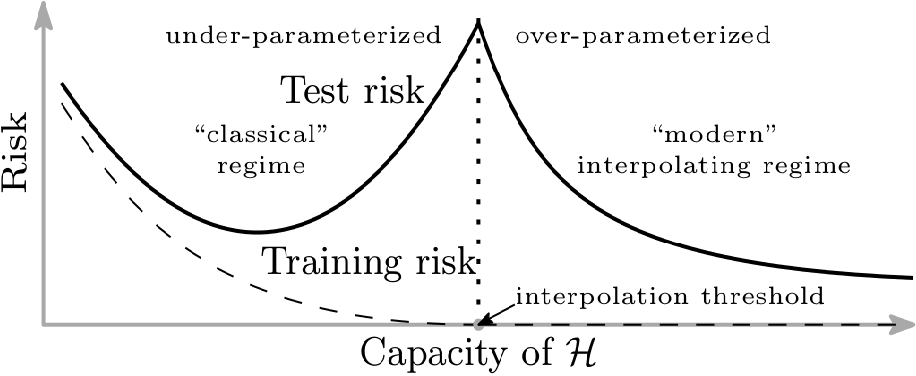
\includegraphics[width=\textwidth]{source/BenignOverfittingModel.png}
\end{frame}

\section{Benign Overfitting}
\subsection{Polynomial fitting}
\begin{frame}{Polynomial fitting}
\begin{block}{unregulated  estimation of \(\theta\)}
given samples \((x_1, y_1), ..., (x_n, y_n)\)

		\begin{equation*}
			X^T = \begin{pmatrix}
			1 & x_1 & ... & x_1^{k-1}\\
			\vdots &&& \vdots\\
			1 & x_n & ... & x_n^{k-1}
			\end{pmatrix} \text{Vandermondematrix}
		\end{equation*}
		
compute \(\theta\) as least square solution of

\begin{equation}
X^T \theta = y
\end{equation}
\end{block}
\end{frame}

\begin{frame}{Polynomial fitting}
\begin{block}{regularized estimation of \(\theta\)}
	problem: \(\min \frac{1}{2} \norm{X^T  \theta -y}^2 + \frac{1}{2} \mu \theta^TW\theta\)
	\vspace{0.5cm}
	\pause
	
	\(\mu\) - weight of regularization term
	
	\(W\) - diagonal matrix, \(w_{ij} := \delta_{ij} i \quad i,j \in \{0,...,k-1\}\)
	\vspace{0.5cm}
	\pause
	
	\(\left(XX^T + \mu W\right) \theta = X y\) \hfill numerically unstable
\end{block}
\end{frame}

\begin{frame}{Polynomial fitting}
	reformulate as: \(\min \frac{1}{2} \norm{\hat{X}^T \theta -\hat{y}}^2\)
	
	\begin{equation*}
		\hat{X} = \begin{pNiceArray}{CCCCC|CCCC}
			\Block{5-5}<\Huge>{X} & & & & & 0 & & ... & 0\\
			& & & & &\sqrt{\mu} & & \Block{2-2}<\huge>{0} &\\
			& & & & & & \sqrt{2\mu} & &\\
			& & & & &\Block{2-2}<\huge>{0} && \ddots &\\
			& & & & & & & & \sqrt{(k-1)\mu}
		\end{pNiceArray}
	\end{equation*}
	
	\begin{equation*}
		\hat{y} = \begin{pmatrix}
			y\\
			0\\
			\vdots\\
			0
		\end{pmatrix}
	\end{equation*}
	
	still solvable using \(QR\) decomposition, but larger matrices

\end{frame}

\begin{frame}{Polynomial fitting examples}
\begin{center}
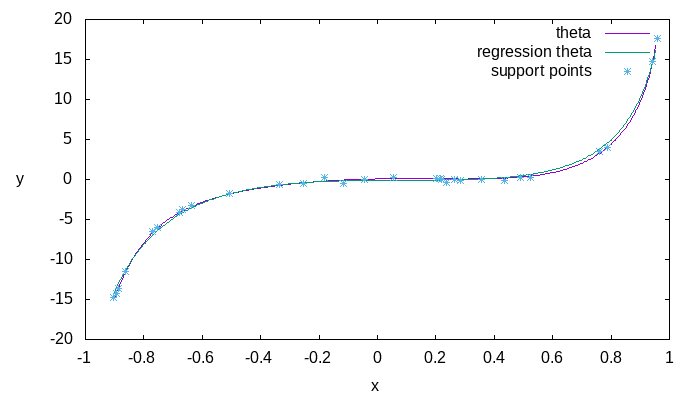
\includegraphics[width=\textwidth]{source/theta_plot_1.png}
\end{center}
\end{frame}

\begin{frame}{Polynomial fitting examples}
\begin{center}
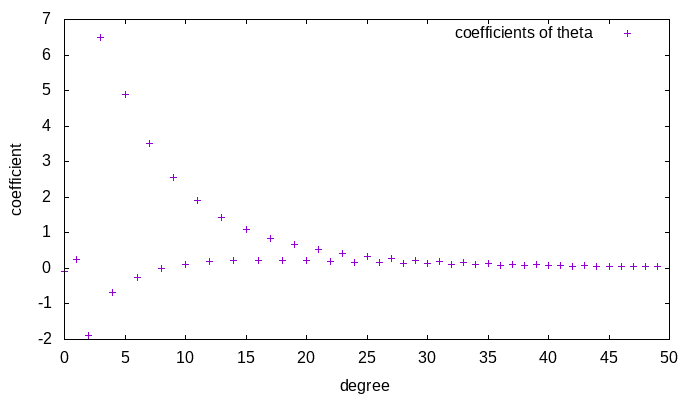
\includegraphics[width=\textwidth]{source/theta_coefficients_1.png}
\end{center}
\end{frame}

\begin{frame}{Polynomial fitting examples}
\begin{center}
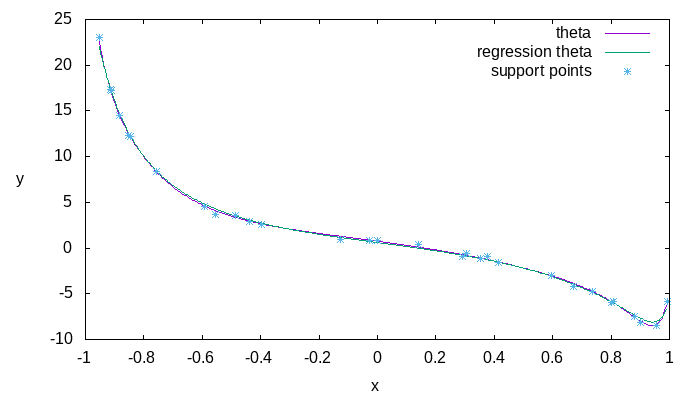
\includegraphics[width=\textwidth]{source/theta_plot_2.png}
\end{center}
\end{frame}

\begin{frame}{Polynomial fitting examples}
\begin{center}
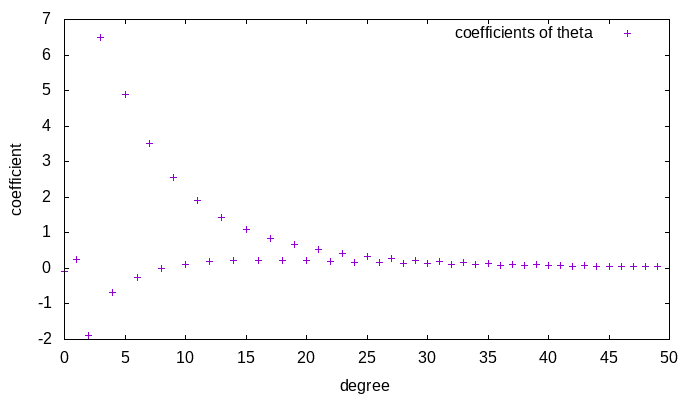
\includegraphics[width=\textwidth]{source/theta_coefficients_1.png}
\end{center}
\end{frame}


\subsection{MNIST}

\begin{frame}{MNIST}
\begin{itemize}
	\item very commonly used benchmark problem in machine learning
	\item goal: recognize hand written digit from an \(28 \cdot 28\) pixel image
	\item contains 60000 training images/ labels, 10000 test images/ labels
	\item standard ML approaches perform very well (\(> 99 \%\) accuracy)
\end{itemize}
\begin{center}
	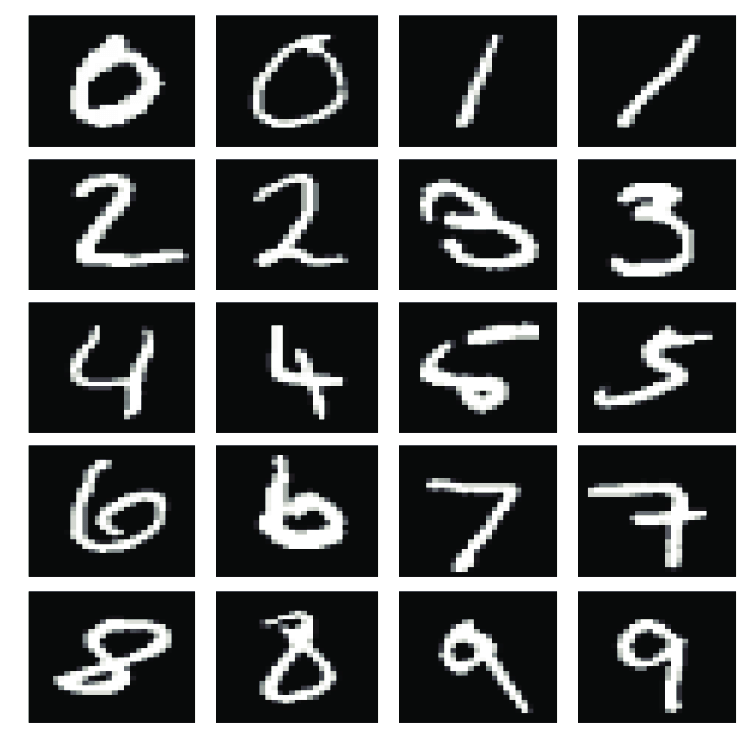
\includegraphics[scale=0.15]{source/mnist.png}
\end{center}
\end{frame}

\begin{frame}{density of accuracy for unregularized optimization}
mean: \(0.8534\) \hfill variance: \(0.0122\)
\begin{center}
	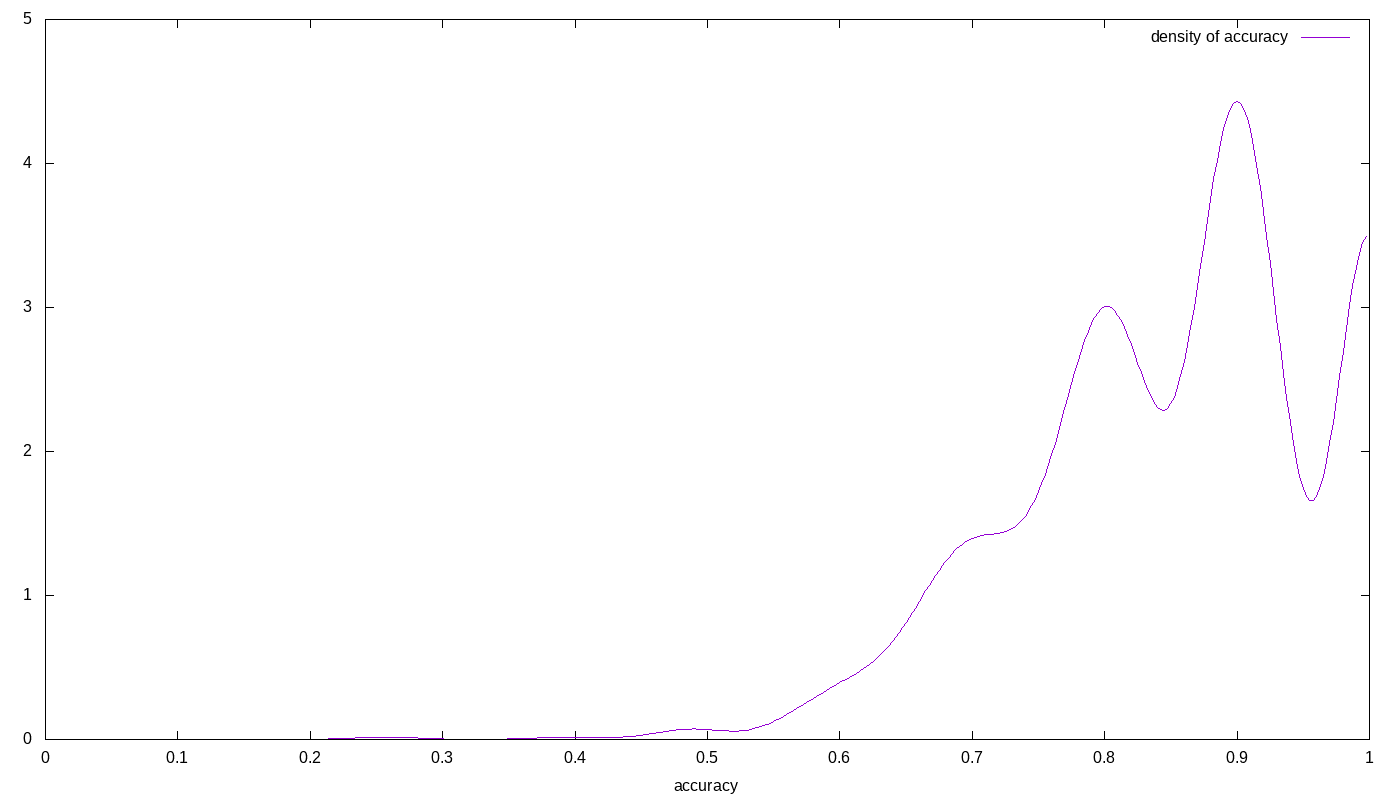
\includegraphics[width=\textwidth]{source/density_unregularized.png}
\end{center}
\end{frame}


\section{Sources}
\begin{frame}{Sources}
\tiny
\begin{itemize}
	\item Bartlett, P. L., Long, P. M., Lugosi, G., \& Tsigler, A. (2020). Benign overfitting in linear regression. Proceedings of the National Academy of Sciences, 117(48), 30063-30070.
	\item \url{http://yann.lecun.com/exdb/mnist/} 13.09.2021 21:45
\end{itemize}
\end{frame}

\begin{frame}{Sources}
\tiny
\begin{itemize}
	\item \url{https://www.researchgate.net/figure/Some-images-in-MNIST-dataset-The-whole-dataset-contains-70-000-2828-gray-scale-images_fig2_330700481} - 11.12.2021 9:58
	\item \url{https://www.catalyzex.com/author/Dino\%20Sejdinovic} 15.12.2021 14:28
\end{itemize}
\end{frame}
\end{document}
